% ============================================================
\chapter{R\'eseaux de neurones artificiels --- Fondements}
\label{ch:reseaux_neurones}
% ============================================================

\begin{intuition}
Un r\'eseau de neurones artificiel est une fonction param\'etrique qui apprend \`a transformer des entr\'ees en sorties en ajustant progressivement ses param\`etres. Comme un enfant qui apprend \`a reconna\^itre des chats en voyant des milliers d'images, le r\'eseau affine ses repr\'esentations internes \`a chaque exemple.
\end{intuition}

% ------------------------------------------------------------
\section{Le neurone formel}
\label{sec:neurone}
\index{neurone formel}

\subsection{Mod\`ele math\'ematique}

Le neurone formel, inspir\'e du mod\`ele de McCulloch-Pitts (1943), calcule une somme pond\'er\'ee de ses entr\'ees suivie d'une fonction d'activation\index{fonction d'activation} :

\begin{mathbox}[title=\textbf{Neurone formel}]
Soit $\bm{x} = (x_1, \ldots, x_d)^\top \in \R^d$ le vecteur d'entr\'ee, $\bm{w} = (w_1, \ldots, w_d)^\top \in \R^d$ le vecteur de poids et $b \in \R$ le biais. La sortie du neurone est :
\[
y = \sigma\!\left(\sum_{i=1}^d w_i x_i + b\right) = \sigma(\bm{w}^\top \bm{x} + b)
\]
o\`u $\sigma : \R \to \R$ est la fonction d'activation.
\end{mathbox}

\begin{center}
\begin{tikzpicture}[
    neuron/.style={circle, draw=NavyBlue, thick, minimum size=1.2cm, fill=blue!10},
    input/.style={circle, draw=gray, thick, minimum size=0.8cm, fill=gray!10},
    >=Stealth
]
% Entrées
\foreach \i/\lab in {1/$x_1$, 2/$x_2$, 3/$x_d$} {
    \node[input] (x\i) at (0, -\i*1.5+1.5) {\lab};
}
\node at (0, -1.5) {$\vdots$};

% Neurone
\node[neuron] (n) at (4, -0.75) {$\sum$, $\sigma$};

% Sortie
\node[right=1.5cm of n] (y) {$y$};

% Connexions
\foreach \i/\w in {1/$w_1$, 2/$w_2$, 3/$w_d$} {
    \draw[->, thick] (x\i) -- node[above, sloped, font=\small] {\w} (n);
}

% Biais
\node[above=0.5cm of n, font=\small] (b) {$b$};
\draw[->, thick] (b) -- (n);

% Sortie
\draw[->, thick] (n) -- (y);
\end{tikzpicture}
\end{center}

\subsection{Fonctions d'activation}
\index{fonction d'activation!sigmo\"ide}
\index{fonction d'activation!ReLU}
\index{fonction d'activation!tanh}

Les fonctions d'activation introduisent la non-lin\'earit\'e essentielle au pouvoir expressif du r\'eseau :

\begin{center}
\begin{tabular}{llll}
\toprule
\textbf{Nom} & \textbf{Formule} & \textbf{Image} & \textbf{Usage} \\
\midrule
Sigmo\"ide & $\sigma(z) = \frac{1}{1+e^{-z}}$ & $(0,1)$ & Sortie binaire \\[6pt]
Tanh & $\tanh(z) = \frac{e^z - e^{-z}}{e^z + e^{-z}}$ & $(-1,1)$ & Couches cach\'ees (historique) \\[6pt]
ReLU & $\relu(z) = \max(0,z)$ & $[0,+\infty)$ & Standard moderne \\[6pt]
Leaky ReLU & $\max(\alpha z, z)$, $\alpha\approx 0.01$ & $\R$ & \'Evite neurones morts \\[6pt]
GELU & $z \cdot \Phi(z)$ & $\R$ & Transformers \\[6pt]
Softmax & $\frac{e^{z_i}}{\sum_j e^{z_j}}$ & $(0,1)^K$ & Classification multi-classe \\
\bottomrule
\end{tabular}
\end{center}

\begin{center}
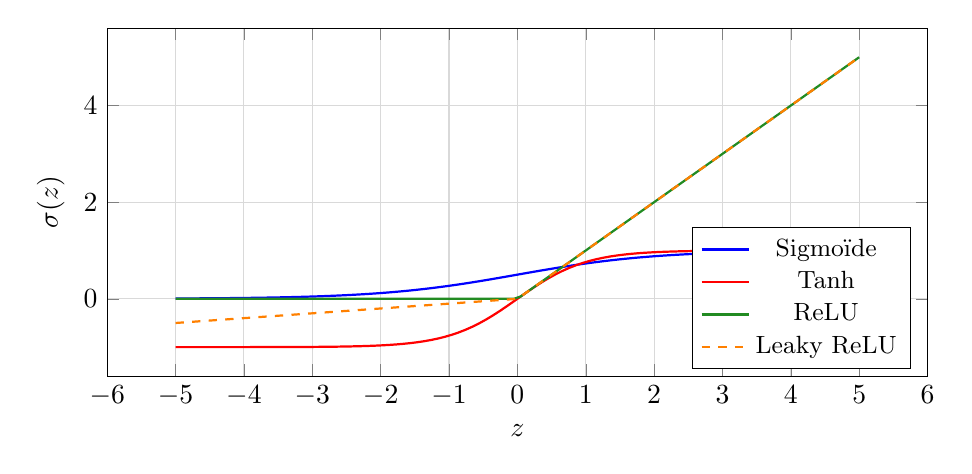
\begin{tikzpicture}
\begin{axis}[
    width=12cm, height=6cm,
    xlabel={$z$}, ylabel={$\sigma(z)$},
    domain=-5:5, samples=100,
    legend style={at={(0.98,0.02)}, anchor=south east, font=\small},
    grid=major, grid style={gray!30}
]
\addplot[blue, thick] {1/(1+exp(-x))}; \addlegendentry{Sigmo\"ide}
\addplot[red, thick] {tanh(x)}; \addlegendentry{Tanh}
\addplot[ForestGreen, thick] {max(0,x)}; \addlegendentry{ReLU}
\addplot[orange, thick, dashed] {x > 0 ? x : 0.1*x}; \addlegendentry{Leaky ReLU}
\end{axis}
\end{tikzpicture}
\end{center}

\begin{attention}
La sigmo\"ide souffre du probl\`eme de \textbf{gradient \'evanescent}\index{gradient \'evanescent} : pour $|z| \gg 0$, $\sigma'(z) \approx 0$, ce qui bloque l'apprentissage dans les couches profondes. C'est pourquoi ReLU est aujourd'hui le choix par d\'efaut.
\end{attention}

% ------------------------------------------------------------
\section{Perceptron multicouche (MLP)}
\label{sec:mlp}
\index{perceptron multicouche}
\index{MLP|see{perceptron multicouche}}

\subsection{Architecture}

Un perceptron multicouche empile $L$ couches de neurones. La couche $\ell$ effectue la transformation :
\[
\bm{h}^{(\ell)} = \sigma^{(\ell)}\!\left(W^{(\ell)} \bm{h}^{(\ell-1)} + \bm{b}^{(\ell)}\right), \quad \ell = 1, \ldots, L
\]
o\`u $\bm{h}^{(0)} = \bm{x}$ est l'entr\'ee et $\bm{h}^{(L)} = \hat{\bm{y}}$ est la sortie.

\begin{definition}[R\'eseau enti\`erement connect\'e]
\label{def:fc}
Un MLP \`a $L$ couches de largeurs $n_0, n_1, \ldots, n_L$ est la composition :
\[
f_\theta(\bm{x}) = \sigma^{(L)} \circ A^{(L)} \circ \sigma^{(L-1)} \circ A^{(L-1)} \circ \cdots \circ \sigma^{(1)} \circ A^{(1)}(\bm{x})
\]
o\`u $A^{(\ell)}(\bm{z}) = W^{(\ell)}\bm{z} + \bm{b}^{(\ell)}$ est une transformation affine avec $W^{(\ell)} \in \R^{n_\ell \times n_{\ell-1}}$, et $\theta = \{W^{(\ell)}, \bm{b}^{(\ell)}\}_{\ell=1}^L$ d\'esigne l'ensemble des param\`etres.
\end{definition}

\begin{center}
\begin{tikzpicture}[
    neuron/.style={circle, draw=NavyBlue, thick, minimum size=0.7cm, fill=blue!10},
    inputn/.style={circle, draw=ForestGreen, thick, minimum size=0.7cm, fill=green!10},
    outputn/.style={circle, draw=BrickRed, thick, minimum size=0.7cm, fill=red!10},
    >=Stealth
]
% Couche d'entrée
\foreach \i in {1,...,4} {
    \node[inputn] (i\i) at (0, -\i*1.2+3) {};
}
\node[below=0.1cm of i4, font=\small, ForestGreen] {Entr\'ee};

% Couche cachée 1
\foreach \i in {1,...,5} {
    \node[neuron] (h1\i) at (3, -\i*1.0+3) {};
}
\node[below=0.1cm of h15, font=\small, NavyBlue] {Couche 1};

% Couche cachée 2
\foreach \i in {1,...,5} {
    \node[neuron] (h2\i) at (6, -\i*1.0+3) {};
}
\node[below=0.1cm of h25, font=\small, NavyBlue] {Couche 2};

% Couche de sortie
\foreach \i in {1,...,3} {
    \node[outputn] (o\i) at (9, -\i*1.2+2.4) {};
}
\node[below=0.1cm of o3, font=\small, BrickRed] {Sortie};

% Connexions
\foreach \i in {1,...,4} {
    \foreach \j in {1,...,5} {
        \draw[gray!40] (i\i) -- (h1\j);
    }
}
\foreach \i in {1,...,5} {
    \foreach \j in {1,...,5} {
        \draw[gray!40] (h1\i) -- (h2\j);
    }
}
\foreach \i in {1,...,5} {
    \foreach \j in {1,...,3} {
        \draw[gray!40] (h2\i) -- (o\j);
    }
}
\end{tikzpicture}
\end{center}

\subsection{Nombre de param\`etres}

Pour un MLP de couches $(n_0, n_1, \ldots, n_L)$, le nombre total de param\`etres est :
\[
|\theta| = \sum_{\ell=1}^{L} (n_{\ell-1} \cdot n_\ell + n_\ell) = \sum_{\ell=1}^{L} n_\ell(n_{\ell-1} + 1)
\]

\begin{exemple}
Un MLP $(784, 256, 128, 10)$ pour MNIST a $784 \times 256 + 256 + 256 \times 128 + 128 + 128 \times 10 + 10 = 235\,146$ param\`etres.
\end{exemple}

% ------------------------------------------------------------
\section{Fonctions de perte}
\label{sec:perte}
\index{fonction de perte}

\subsection{R\'egression : erreur quadratique moyenne}
\index{MSE|see{erreur quadratique moyenne}}

Pour la r\'egression, on minimise l'erreur quadratique moyenne (MSE) :
\[
\mathcal{L}_{\mathrm{MSE}}(\theta) = \frac{1}{N} \sum_{i=1}^{N} \|\bm{y}_i - f_\theta(\bm{x}_i)\|^2
\]

\subsection{Classification : entropie crois\'ee}
\index{entropie crois\'ee}

Pour la classification \`a $K$ classes avec sortie softmax :
\[
\mathcal{L}_{\mathrm{CE}}(\theta) = -\frac{1}{N}\sum_{i=1}^{N} \sum_{k=1}^{K} y_{ik} \log \hat{y}_{ik}
\]
o\`u $y_{ik} \in \{0,1\}$ est l'encodage one-hot et $\hat{y}_{ik} = \softmax(z_{ik})$.

\begin{mathbox}[title=\textbf{Lien avec le maximum de vraisemblance}]
Minimiser l'entropie crois\'ee est \'equivalent \`a maximiser la log-vraisemblance sous un mod\`ele cat\'egorique :
\[
\hat{\theta}_{\mathrm{MLE}} = \argmax_\theta \sum_{i=1}^N \log p(y_i \mid \bm{x}_i; \theta) = \argmin_\theta \mathcal{L}_{\mathrm{CE}}(\theta)
\]
\end{mathbox}

\subsection{Classification binaire : entropie crois\'ee binaire}
\index{entropie crois\'ee!binaire}

Pour $K=2$ avec sortie sigmo\"ide :
\[
\mathcal{L}_{\mathrm{BCE}}(\theta) = -\frac{1}{N}\sum_{i=1}^{N} \left[y_i \log \hat{y}_i + (1-y_i)\log(1-\hat{y}_i)\right]
\]

% ------------------------------------------------------------
\section{Th\'eor\`eme d'approximation universelle}
\label{sec:uat}
\index{approximation universelle}

\begin{theoreme}[Cybenko, 1989 ; Hornik, 1991]
\label{thm:uat}
Soit $\sigma$ une fonction d'activation continue et non polynomiale. Pour toute fonction continue $f : [0,1]^d \to \R$ et tout $\varepsilon > 0$, il existe $n \in \N$, des poids $w_{ij}, b_j, c_j$ tels que :
\[
\left| f(\bm{x}) - \sum_{j=1}^{n} c_j \, \sigma\!\left(\sum_{i=1}^d w_{ij} x_i + b_j\right) \right| < \varepsilon \quad \forall \bm{x} \in [0,1]^d
\]
\end{theoreme}

\begin{intuition}
Le th\'eor\`eme d'approximation universelle dit qu'un MLP \`a une seule couche cach\'ee \emph{suffisamment large} peut approximer toute fonction continue. Cependant, il ne dit rien sur :
\begin{itemize}
\item La \textbf{largeur} $n$ n\'ecessaire (qui peut \^etre exponentiellement grande).
\item La \textbf{facilit\'e d'apprentissage} des poids optimaux.
\item L'avantage de la \textbf{profondeur} (couches multiples) par rapport \`a la largeur.
\end{itemize}
En pratique, les r\'eseaux profonds atteignent de meilleures performances avec beaucoup moins de param\`etres que les r\'eseaux larges et peu profonds.
\end{intuition}

% ------------------------------------------------------------
\section{Initialisation des poids}
\label{sec:init}
\index{initialisation des poids}
\index{Xavier|see{initialisation des poids}}
\index{He|see{initialisation des poids}}

Une mauvaise initialisation peut provoquer l'explosion ou l'\'evanescence des activations d\`es la passe avant.

\begin{mathbox}[title=\textbf{Initialisation de Xavier/Glorot (2010)}]
Pour pr\'eserver la variance des activations \`a travers les couches avec des activations sym\'etriques (tanh, sigmo\"ide lin\'eaire) :
\[
W^{(\ell)}_{ij} \sim \mathcal{U}\!\left(-\sqrt{\frac{6}{n_{\ell-1}+n_\ell}}, \sqrt{\frac{6}{n_{\ell-1}+n_\ell}}\right)
\]
\end{mathbox}

\begin{mathbox}[title=\textbf{Initialisation de He/Kaiming (2015)}]
Pour les activations ReLU (qui annulent la moiti\'e des activations) :
\[
W^{(\ell)}_{ij} \sim \mathcal{N}\!\left(0, \frac{2}{n_{\ell-1}}\right)
\]
\end{mathbox}

% ------------------------------------------------------------
\section{Impl\'ementation PyTorch}
\label{sec:impl_mlp}

\begin{codeblock}[title=\textbf{MLP en PyTorch --- Classification MNIST}]
\begin{minted}{python}
import torch
import torch.nn as nn
import torch.optim as optim
from torchvision import datasets, transforms
from torch.utils.data import DataLoader

# Hyperparamètres
BATCH_SIZE = 128
LR = 1e-3
EPOCHS = 10
DEVICE = torch.device('cuda' if torch.cuda.is_available() else 'cpu')

# Données MNIST
transform = transforms.Compose([
    transforms.ToTensor(),
    transforms.Normalize((0.1307,), (0.3081,))
])
train_data = datasets.MNIST('./data', train=True, download=True,
                            transform=transform)
test_data = datasets.MNIST('./data', train=False, transform=transform)
train_loader = DataLoader(train_data, batch_size=BATCH_SIZE, shuffle=True)
test_loader = DataLoader(test_data, batch_size=BATCH_SIZE)

# Modèle MLP
class MLP(nn.Module):
    def __init__(self, input_dim=784, hidden_dims=[256, 128],
                 num_classes=10):
        super().__init__()
        layers = []
        prev = input_dim
        for h in hidden_dims:
            layers += [nn.Linear(prev, h), nn.ReLU()]
            prev = h
        layers.append(nn.Linear(prev, num_classes))
        self.net = nn.Sequential(*layers)

    def forward(self, x):
        return self.net(x.view(x.size(0), -1))  # Aplatir

model = MLP().to(DEVICE)
print(f"Paramètres : {sum(p.numel() for p in model.parameters()):,}")

# Entraînement
criterion = nn.CrossEntropyLoss()
optimizer = optim.Adam(model.parameters(), lr=LR)

for epoch in range(1, EPOCHS + 1):
    model.train()
    total_loss = 0
    for X, y in train_loader:
        X, y = X.to(DEVICE), y.to(DEVICE)
        optimizer.zero_grad()
        loss = criterion(model(X), y)
        loss.backward()
        optimizer.step()
        total_loss += loss.item() * X.size(0)

    # Évaluation
    model.eval()
    correct = 0
    with torch.no_grad():
        for X, y in test_loader:
            X, y = X.to(DEVICE), y.to(DEVICE)
            correct += (model(X).argmax(1) == y).sum().item()

    acc = correct / len(test_data)
    print(f"Epoch {epoch:2d} | Loss: {total_loss/len(train_data):.4f}"
          f" | Test Acc: {acc:.4f}")
\end{minted}
\end{codeblock}

\begin{codeoutput}
\begin{verbatim}
Paramètres : 235,146
Epoch  1 | Loss: 0.2534 | Test Acc: 0.9612
Epoch  2 | Loss: 0.1042 | Test Acc: 0.9710
...
Epoch 10 | Loss: 0.0198 | Test Acc: 0.9793
\end{verbatim}
\end{codeoutput}

% ------------------------------------------------------------
\section{\'Etude d'ablation : influence de la largeur et de la profondeur}
\label{sec:ablation_mlp}

\begin{codeblock}[title=\textbf{\'Etude d'ablation}]
\begin{minted}{python}
# Comparaison de différentes architectures MLP sur MNIST
configs = {
    "Shallow-wide":  [1024],
    "2-layers":      [256, 128],
    "3-layers":      [256, 128, 64],
    "Deep-narrow":   [64, 64, 64, 64],
}

results = {}
for name, hidden in configs.items():
    model = MLP(hidden_dims=hidden).to(DEVICE)
    n_params = sum(p.numel() for p in model.parameters())
    # ... entraîner et évaluer ...
    results[name] = {"params": n_params, "acc": test_acc}
    print(f"{name:20s} | {n_params:>8,} params | Acc: {test_acc:.4f}")
\end{minted}
\end{codeblock}

\begin{codeoutput}
\begin{verbatim}
Shallow-wide         |  812,042 params | Acc: 0.9781
2-layers             |  235,146 params | Acc: 0.9793
3-layers             |  243,338 params | Acc: 0.9802
Deep-narrow          |   63,434 params | Acc: 0.9745
\end{verbatim}
\end{codeoutput}

\begin{remarque}
L'architecture \`a 3 couches atteint la meilleure pr\'ecision avec un nombre raisonnable de param\`etres. Le r\'eseau large et peu profond utilise 3$\times$ plus de param\`etres pour un r\'esultat similaire. Le r\'eseau profond et \'etroit, bien qu'\'economique, perd en performance --- la largeur minimale par couche importe.
\end{remarque}

% ------------------------------------------------------------
\section{Connexion \`a l'\'etat de l'art}
\label{sec:sota_mlp}

\begin{sota}
\begin{itemize}
\item \textbf{MLP-Mixer} (Tolstikhin et al., 2021) : architecture enti\`erement MLP pour la vision, rivalisant avec les CNN et les ViT en utilisant uniquement des m\'elanges de tokens et de canaux.
\item \textbf{KAN} (Kolmogorov-Arnold Networks, Liu et al., 2024) : remplacent les poids fixes par des fonctions apprenables sur les ar\^etes, am\'eliorant l'interpr\'etabilit\'e et l'efficacit\'e sur des probl\`emes scientifiques.
\item \textbf{Scaling laws} (Kaplan et al., 2020) : la performance d'un r\'eseau suit des lois de puissance en fonction du nombre de param\`etres, de la taille des donn\'ees et du budget de calcul.
\end{itemize}
\end{sota}

% ------------------------------------------------------------
\section{R\'esum\'e du chapitre}

\begin{formules}
\begin{itemize}
\item \textbf{Neurone formel} : $y = \sigma(\bm{w}^\top \bm{x} + b)$
\item \textbf{MLP} : $f_\theta = \sigma^{(L)} \circ A^{(L)} \circ \cdots \circ \sigma^{(1)} \circ A^{(1)}$
\item \textbf{Perte MSE} : $\frac{1}{N}\sum_i \|y_i - \hat{y}_i\|^2$
\item \textbf{Perte CE} : $-\frac{1}{N}\sum_i \sum_k y_{ik}\log\hat{y}_{ik}$
\item \textbf{Init Xavier} : $W \sim \mathcal{U}(-\sqrt{6/(n_{\mathrm{in}}+n_{\mathrm{out}})}, +\cdot)$
\item \textbf{Init He} : $W \sim \mathcal{N}(0, 2/n_{\mathrm{in}})$
\item \textbf{UAT} : un MLP \`a 1 couche cach\'ee peut approximer toute fonction continue
\end{itemize}
\end{formules}

% ------------------------------------------------------------
\section{Exercices}

\begin{exercice}[$\star$ --- D\'erivation]
Montrer que la d\'eriv\'ee de la sigmo\"ide v\'erifie $\sigma'(z) = \sigma(z)(1 - \sigma(z))$. En d\'eduire que $\max_z \sigma'(z) = 1/4$.
\end{exercice}

\begin{exercice}[$\star$ --- Comptage de param\`etres]
Calculer le nombre exact de param\`etres d'un MLP $(1024, 512, 256, 128, 10)$. Comparer avec un r\'eseau $(1024, 2048, 10)$ de m\^eme budget param\'etrique approximatif.
\end{exercice}

\begin{exercice}[$\star\star$ --- Impl\'ementation]
Impl\'ementer un MLP en PyTorch pour la classification Fashion-MNIST (10 classes de v\^etements). Comparer les performances avec ReLU, Leaky ReLU et GELU. Tracer les courbes d'apprentissage.
\end{exercice}

\begin{exercice}[$\star\star$ --- \'Etude d'ablation]
R\'ealiser une \'etude d'ablation syst\'ematique sur MNIST en faisant varier : (a) le nombre de couches de 1 \`a 6, (b) la largeur de 32 \`a 512. Tracer une carte de chaleur (heatmap) pr\'ecision vs (profondeur, largeur).
\end{exercice}

\begin{exercice}[$\star\star\star$ --- Projet de recherche]
Impl\'ementer un MLP-Mixer pour CIFAR-10 en suivant l'article de Tolstikhin et al. (2021). Comparer ses performances avec un MLP classique et un CNN simple. Analyser l'influence de la taille des patchs et de la dimension cach\'ee.
\end{exercice}
